\documentclass[tikz,border=5pt]{standalone}
\usepackage{amsmath,amssymb,mathtools}
\usepackage{braket}
\usepackage{xcolor}
\usepackage{tikz}
\usetikzlibrary{arrows.meta,decorations.pathmorphing,decorations.pathreplacing,calc,positioning}

\definecolor{cobalt}{HTML}{2b4c7e}
\definecolor{boxblue}{HTML}{eef3fa}
\definecolor{boxgold}{HTML}{fbf3e3}
\definecolor{boxred}{HTML}{fbecec}
\definecolor{boxgreen}{HTML}{eaf6f0}
\definecolor{ruleblue}{HTML}{2b6cb0}
\definecolor{rulegold}{HTML}{b7791f}
\definecolor{rulered}{HTML}{c0392b}
\definecolor{rulegreen}{HTML}{1f8a5f}

\newcommand{\HH}{\mathcal{H}}
\newcommand{\M}{\mathcal{M}}
\newcommand{\tr}{\operatorname{tr}}
\newcommand{\Tr}{\operatorname{Tr}}
\newcommand{\ii}{\mathrm{i}}
\begin{document}
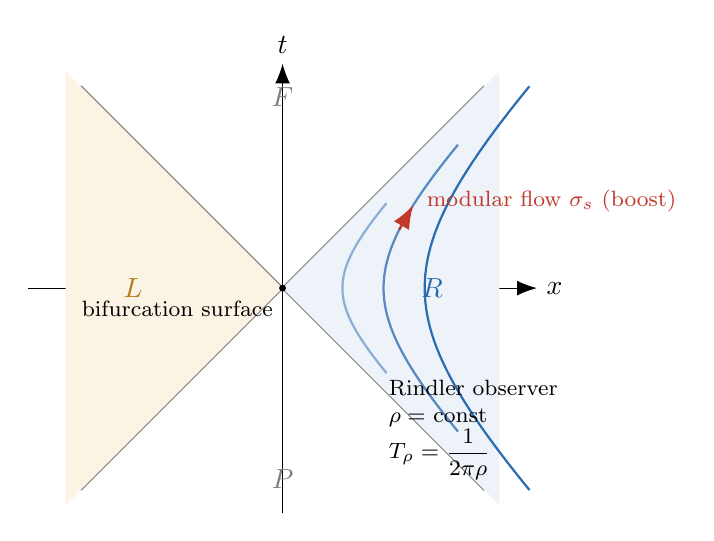
\begin{tikzpicture}[scale=0.95, >=Latex]
  % axes
  \draw[-{Latex[length=2.5mm]}] (-3.4,0) -- (3.4,0) node[right] {$x$};
  \draw[-{Latex[length=2.5mm]}] (0,-3.0) -- (0,3.0) node[above] {$t$};
  % lightcones through origin
  \draw[thick, gray] (-2.7,-2.7) -- (2.7,2.7);
  \draw[thick, gray] (-2.7,2.7) -- (2.7,-2.7);
  % shade right (R) and left (L) wedges
  \begin{scope}
    \clip (0,0) -- (2.9,2.9) -- (2.9,-2.9) -- cycle;
    \fill[boxblue] (-3,-3) rectangle (3,3);
  \end{scope}
  \begin{scope}
    \clip (0,0) -- (-2.9,2.9) -- (-2.9,-2.9) -- cycle;
    \fill[boxgold] (-3,-3) rectangle (3,3);
  \end{scope}
  \node[ruleblue] at (2.0,0) {\textbf{$R$}};
  \node[rulegold] at (-2.0,0) {\textbf{$L$}};
  \node[gray] at (0,2.55) {$F$};
  \node[gray] at (0,-2.55) {$P$};
  % Rindler hyperbolas rho = const in R wedge:  x^2 - t^2 = rho^2
  \foreach \rho/\col in {0.8/ruleblue!55, 1.35/ruleblue!80, 1.9/ruleblue}{
    \draw[thick, \col, domain=-1.15:1.15, samples=60, variable=\e]
      plot ({\rho*cosh(\e)}, {\rho*sinh(\e)});
  }
  % boost flow arrow along rho=1.35 hyperbola, at e=0.55
  \pgfmathsetmacro{\ea}{0.55}
  \pgfmathsetmacro{\xa}{1.35*cosh(\ea)}
  \pgfmathsetmacro{\ya}{1.35*sinh(\ea)}
  \pgfmathsetmacro{\eb}{0.75}
  \pgfmathsetmacro{\xb}{1.35*cosh(\eb)}
  \pgfmathsetmacro{\yb}{1.35*sinh(\eb)}
  \draw[-{Latex[length=3mm]}, rulered, thick] (\xa,\ya) -- (\xb,\yb);
  \node[rulered, right] at (\xb+0.05,\yb+0.05) {\footnotesize modular flow $\sigma_s$ (boost)};
  % redshift/temperature label
  \node[align=left, font=\footnotesize] at (2.55,-1.9) {Rindler observer\\ $\rho=$ const\\ $T_\rho=\dfrac{1}{2\pi\rho}$};
  % origin bifurcation point
  \fill[black] (0,0) circle (1.3pt);
  \node[below left, font=\footnotesize] at (0,-0.05) {bifurcation surface};
\end{tikzpicture}

\end{document}
